\mySection{5.2 Estimating parameters: MLE and MME}
%-------------- start slide -------------------------------%{{{ 5.10
\begin{frame}
  % {\S\: 5.2 Estimating parameters: MLE and MME}

{\bf\noindent Two methods} for estimating parameters \hfill Corresponding estimator
\vspace{2em}
\begin{enumerate}
 \item Method of maximum likelihood.\hfill MLE \hspace{3em}\phantom{a}
 \vspace{2em}
 \item Method of moments.\hfill MME \hspace{3em}\phantom{a}
\end{enumerate}

% \vf
\end{frame}
%-------------- end slide -------------------------------%}}}
%-------------- start slide -------------------------------%{{{ 5.11
\begin{frame}{Maximum Likelihood Estimation}

{\bf\noindent Definition 5.2.1.~} For a random sample of size $n$ from the
discrete (resp. continuous) population/pdf $p_X(k;\theta)$ (resp.
$f_Y(y;\theta)$), the \textcolor{yellow}{likelihood function}, $L(\theta)$, is the product of
the pdf evaluated at $X_i=k_i$ (resp. $Y_i=y_i$), i.e., \[ L(\theta) =
\prod_{i=1}^n p_X(k_i;\theta) \qquad \bigg(\text{resp.}\: L(\theta) =
\prod_{i=1}^n f_Y(y_i;\theta) \bigg).  \]

\pause \vfill {\bf\noindent Definition 5.2.2.~} Let $L(\theta)$ be as defined
in Definition 5.2.1. If $\theta_e$ is a value of the parameter such that
$L(\theta_e)\ge L(\theta)$ for all possible values of $\theta$, then we call
$\theta_e$ the \textcolor{yellow}{maximum likelihood estimate} for $\theta$.
\end{frame}
%-------------- end slide -------------------------------%}}}
%-------------- start slide -------------------------------%{{{ 5.12
\begin{frame}{Examples for MLE}
Often but not always MLE can be obtained by setting the first derivative equal to zero:\\
\vfill
\begin{enumerate}
 \item[E.g. 1.] Poisson distribution: $p_X(k) = e^{-\lambda}\frac{\lambda^k}{k!}$, $k=0,1,\cdots$.
 \[
 L(\lambda) = \prod_{i=1}^n
e^{-\lambda}\frac{\lambda^{k_i}}{k_i!} = e^{-n\lambda} \lambda^{\sum_{i=1}^k k_i}\left(\prod_{i=1}^n
 k_i!\right)^{-1}.
 \]\pause
 \[
 \ln L(\lambda) = -n\lambda + \left(\sum_{i=1}^{n} k_i\right)\ln \lambda - \ln\left(\prod_{i=1}^{n}k_i!\right).
 \]\pause
 \[
 \frac{\ud }{\ud \lambda} \ln L(\lambda) =  - n + \frac{1}{\lambda}\sum_{i=1}^n k_i.
 \]\pause
 \[
 \frac{\ud }{\ud \lambda} \ln L(\lambda) =0 \quad\Longrightarrow\quad
 \boxed{\lambda_e = \frac{1}{n}\sum_{i=1}^n k_i =: \bar{k}}.
 \]\pause
 \vfill
 {Comment:~} The critical point is indeed global maximum because
 \[
 \frac{\ud^2 }{\ud \lambda^2} \ln L(\lambda) =  - \frac{1}{\lambda^2}\sum_{i=1}^n k_i<0.
 \]
 \end{enumerate}
\end{frame}
%-------------- end slide -------------------------------%}}}
%-------------- start slide -------------------------------%{{{ 5.13
\begin{frame}

The following two cases are related to waiting time: \\[1em]

 \begin{enumerate}
 \item[E.g. 2.] Exponential distribution: $f_Y(y)=\lambda e^{-\lambda y}$ for $y\ge 0$.
 \[
 L(\lambda) = \prod_{i=1}^n
\lambda e^{-\lambda y_i} = \lambda^{n} \exp\left(-\lambda\sum_{i=1}^n y_i\right)
 \]\pause
 \[
 \ln L(\lambda) = n\ln\lambda - \lambda\sum_{i=1}^n y_i.
 \]\pause
 \[
 \frac{\ud }{\ud \lambda} \ln L(\lambda) =   \frac{n}{\lambda} - \sum_{i=1}^n y_i.
 \]\pause
 \[
 \frac{\ud }{\ud \lambda} \ln L(\lambda) =0 \quad\Longrightarrow\quad
 \boxed{\lambda_e = \frac{n}{\sum_{i=1}^n y_i} =: \frac{1}{\bar{y} }}.
 \]
\end{enumerate}

\end{frame}
%-------------- end slide -------------------------------%}}}
%-------------- start slide -------------------------------%{{{ 5.14
\begin{frame}
A random sample of size $n$ from the following population: \\[1em]
 \begin{enumerate}
 \item[E.g. 3.] Gamma distribution: $f_Y(y;\lambda)= \frac{\lambda^r}{\Gamma(r)} y^{r-1} e^{-\lambda y}$ for $y\ge 0$ with $r>1$ known.
 \[
 L(\lambda) = \prod_{i=1}^n
\frac{\lambda^r}{\Gamma(r)} y_i^{r-1} e^{-\lambda y_i} = \lambda^{r \: n} \Gamma(r)^{{-n}} \left(\prod_{i=1}^n y_i^{r-1}\right)\exp\left(-\lambda\sum_{i=1}^n y_i\right)
 \]\pause
 \[
 \ln L(\lambda) = r\: n\ln\lambda -n\ln\Gamma(r)+ \ln\left(\prod_{i=1}^{n}y_i^{r-1}\right)-\lambda\sum_{i=1}^n y_i.
 \]\pause
 \[
 \frac{\ud }{\ud \lambda} \ln L(\lambda) =   \frac{r\: n}{\lambda} -\sum_{i=1}^n y_i.
 \]\pause
 \[
 \frac{\ud }{\ud \lambda} \ln L(\lambda) =0 \quad\Longrightarrow\quad
 \boxed{\lambda_e = \frac{r\: n}{\sum_{i=1}^n y_i} = \frac{r}{\bar{y} }}.
 \]
 \vfill
 Comment:
 \begin{itemize}
  \item When $r=1$, this reduces to the exponential distribution case.
  \item If $r$ is also unknown, it will be much more complicated.\\
  No closed-form solution. One needs numerical solver\footnote{[DW, Example 7.2.25]}.\\
  Try MME instead.
 \end{itemize}
\end{enumerate}
\end{frame}
%-------------- end slide -------------------------------%}}}
%-------------- start slide -------------------------------%{{{ 5.15
\begin{frame}
  A detailed study with data: \\[1em]
 \begin{enumerate}
 \item[E.g. 4.] Geometric distribution: $p_X(k;p)=  (1-p)^{k-1} p$, $k=1,2,\cdots$.
 \[
 L(p) = \prod_{i=1}^n (1-p)^{k_i-1} p
 = (1-p)^{-n+ \sum_{i=1}^k k_i }p^n.
 \]\pause
 \[
 \ln L(p) = \left(-n+\sum_{i=1}^n k_i\right) \ln(1-p) + n\ln p.
 \]\pause
 \[
 \frac{\ud }{\ud p} \ln L(p) =  -\frac{-n+\sum_{i=1}^n k_i}{1-p} +\frac{n}{p}.
 \]\pause
 \[
 \frac{\ud }{\ud p} \ln L(p) =0 \quad\Longrightarrow\quad
 \boxed{p_e= \frac{n}{\sum_{i=1}^n k_i} = \frac{1}{\bar{k} }}.
 \]\pause
\vfill
Comment: Its cousin distribution, the negative binomial distribution can be worked out similarly (See Ex 5.2.14).
 \end{enumerate}
\end{frame}
%-------------- end slide -------------------------------%}}}
%-------------- start slide -------------------------------%{{{ 5.16
\begin{frame}
	\begin{center}
		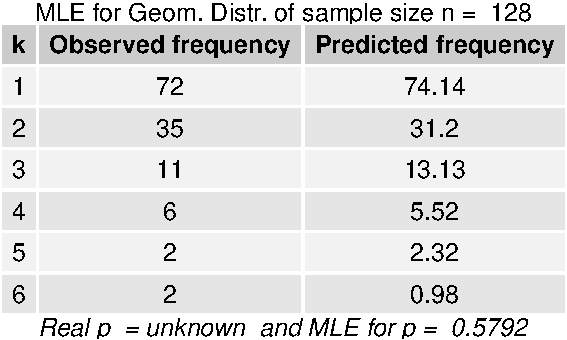
\includegraphics[scale=0.7]{Geometric.pdf}
	\end{center}
\end{frame}
%-------------- end slide -------------------------------%}}}
%-------------- start slide -------------------------------%{{{ 5.17
\begin{frame}[fragile]

 \begin{lstlisting}
# The example from the book.
library(pracma) # Load the library "Practical Numerical Math Functions"
k<-c(72, 35, 11, 6, 2, 2) # observed freq.
a=1:6
pe=sum(k)/dot(k,a) # MLE for p.
f=a
for (i in 1:6) {
  f[i] = round((1-pe)^(i-1) * pe * sum(k),2)
}
# Initialize the table
d <-matrix(1:18, nrow = 6, ncol = 3)
# Now adding the column names
colnames(d) <- c("k",
                 "Observed freq.",
                 "Predicted freq.")
d[1:6,1]<-a
d[1:6,2]<-k
d[1:6,3]<-f
grid.table(d) # Show the table
PlotResults("unknown", pe, d, "Geometric.pdf") # Output the results using a user defined function
\end{lstlisting}
\end{frame}
%-------------- end slide -------------------------------%}}}
%-------------- start slide -------------------------------%{{{ 5.18
\begin{frame}
	\begin{center}
		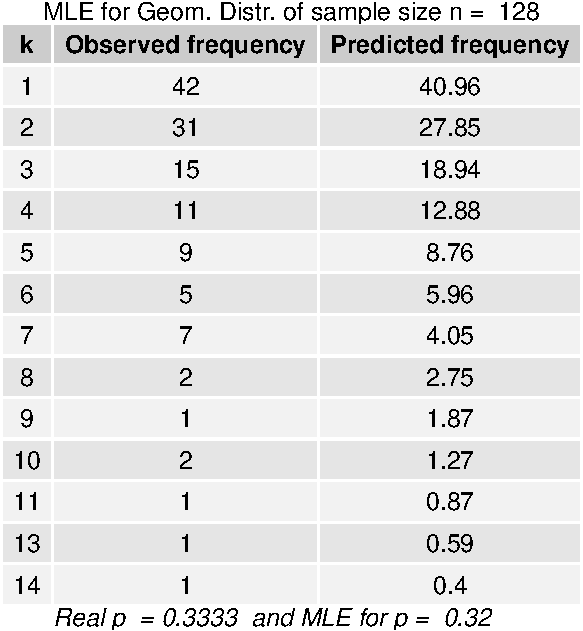
\includegraphics[scale=0.7]{Geometric2.pdf}
	\end{center}
\end{frame}
%-------------- end slide -------------------------------%}}}
%-------------- start slide -------------------------------%{{{ 5.19
\begin{frame}[fragile]

 \begin{lstlisting}
# Now let's generate random samples from a Geometric distribution with p=1/3 with the same size of the sample.
p = 1/3
n = 128
gdata<-rgeom(n, p)+1 # Generate random samples
g<- table(gdata) # Count frequency of your data.
g<- t(rbind(as.numeric(rownames(g)), g)) # Transpose and combine two columns.
pe=n/dot(g[,1],g[,2]) # MLE for p.
f <- g[,1] # Initialize f
for (i in 1:nrow(g)) {
  f[i] = round((1-pe)^(i-1) * pe * n,2)
} # Compute the expected frequency
g<-cbind(g,f) # Add one columns to your matrix.
colnames(g) <- c("k",
                 "Observed freq.",
                 "Predicted freq.") # Specify the column names.
d_df <- as.data.frame(d) # One can use data frame to store data
d_df # Show data on your terminal
PlotResults(p, pe, g, "Geometric2.pdf") # Output the results using a user defined function
 \end{lstlisting}

\end{frame}
%-------------- end slide -------------------------------%}}}
%-------------- start slide -------------------------------%{{{ 5.20
\begin{frame}
	\begin{center}
		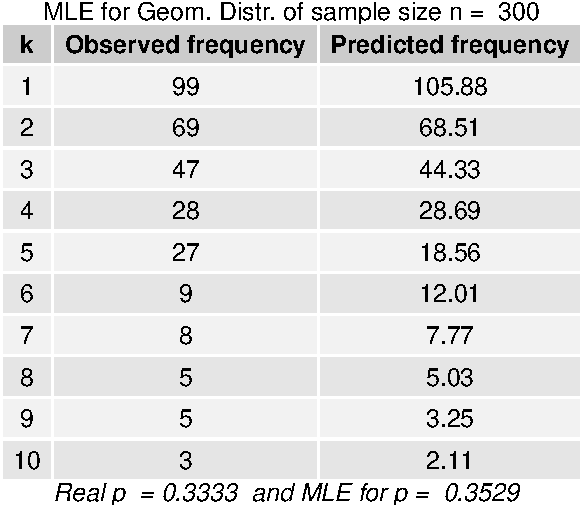
\includegraphics[scale=0.7]{Geometric3.pdf}
	\end{center}
\end{frame}
%-------------- end slide -------------------------------%}}}
%-------------- start slide -------------------------------%{{{ 5.21
\begin{frame}


In case we have several parameters:
\vfill

 \begin{enumerate}
 \item[E.g. 5.] Normal distribution: $f_Y(y;\mu,\sigma^2)= \frac{1}{\sqrt{2\pi} \sigma} e^{-\frac{(y-\mu)^2}{2\sigma^2}}$, $y\in\R$.
 \[
 L(\mu,\sigma^2) = \prod_{i=1}^n \frac{1}{\sqrt{2\pi} \sigma} e^{-\frac{(y_i-\mu)^2}{2\sigma^2}}
 = (2\pi\sigma^2)^{-n/2} \exp\left(-\frac{1}{2\sigma^2}\sum_{i=1}^n(y_i-\mu)^2 \right)
 \]\pause
 \[
 \ln L(\mu,\sigma^2) = -\frac{n}{2}\ln(2\pi\sigma^2) -\frac{1}{2\sigma^2}\sum_{i=1}^n (y_i-\mu)^2.
 \]\pause
 \[
 \begin{cases}
  \displaystyle \frac{\partial }{\partial \mu} \ln L(\mu,\sigma^2) = \frac{1}{\sigma^2}\sum_{i=1}^n
(y_i-\mu) \\
\displaystyle  \frac{\partial }{\partial \sigma^2} \ln L(\mu,\sigma^2) = -\frac{n}{2\sigma^2}+\frac{1}{2\sigma^4}\sum_{i=1}^n(y_i-\mu)^2
\end{cases}
 \]\pause
 \[
 \begin{cases}
  \displaystyle \frac{\partial }{\partial \mu} \ln L(\mu,\sigma^2) = 0\\
\displaystyle  \frac{\partial }{\partial \sigma^2} \ln L(\mu,\sigma^2) =0
\end{cases}
\quad\Longrightarrow\quad
\boxed{\begin{cases}
 \displaystyle \mu_e=\bar{y}\\
 \displaystyle  \sigma_e^2=\frac{1}{n}\sum_{i=1}^n(y_i-\bar{y})^2
\end{cases}}
 \]
\end{enumerate}

\end{frame}
%-------------- end slide -------------------------------%}}}
%-------------- start slide -------------------------------%{{{ 5.22
\begin{frame}
In case when the parameters determine the support of the density:\\
(Non regular case)
\vfill

 \begin{enumerate}
 \item[E.g. 6.] Uniform distribution on $[a,b]$ with $a<b$: $f_Y(y;a,b)=\frac{1}{b-a}$ if $y\in [a,b]$.
 \[
 L(a,b) =
 \begin{cases}
  \prod_{i=1}^n \frac{1}{b-a} =\frac{1}{(b-a)^n}  & \text{if $a\le y_1,\cdots,y_n\le b$,}\\
  0  & \text{otherwise.}
 \end{cases}
 \]\pause
 $L(a,b)$ is monotone increasing in $a$ and decreasing in $b$. Hence, in order to maximize $L(a,b)$,
 one needs to choose
 \[
  a_e=y_{min} \quad\text{and}\quad b_e=y_{max}.
 \]\pause
 \vfill
  \item[E.g. 7.] $f_Y(y;\theta) = \frac{2y}{\theta^2}$ for $y\in [0,\theta]$.
  \[
 L(\theta) =
 \begin{cases}
  \prod_{i=1}^n \frac{2y_i}{\theta^2} =2^n \theta^{-2n}\prod_{i=1}^n y_i  & \text{if $0\le y_1,\cdots,y_n\le \theta$,}\\
  0  & \text{otherwise.}
 \end{cases}
  \]\pause
  \[
  \Downarrow
  \]
  \[
  \theta_e = y_{max}.
  \]
  \end{enumerate}
\end{frame}
%-------------- end slide -------------------------------%}}}
%-------------- start slide -------------------------------%{{{ 5.23
\begin{frame}[fragile]
In case of discrete parameter:
\vfill
\begin{enumerate}
 \item[E.g. 8.] {\bf Wildlife sampling.}  Capture-tag-recapture.... In the history, $a$ tags have been put.
 In order to estimate the population size $N$, one randomly captures $n$ animals, and there are $k$ tagged. Find the MLE for $N$.\\
 \vfill
 {\bf Sol.}
 The population follows hypergeometric distr.: $p_X(k;N)=\frac{{a\choose k}{N-a\choose n-k}}{{N\choose n}}$.\\ \pause
 \[
 L(N) = \frac{{a\choose k}{N-a\choose n-k}}{{N\choose n}}
 \]\pause
 How to maximize $L(N)$? \\ \pause
 \begin{minipage}{0.4\textwidth}
 \begin{lstlisting}
> a=10
> k=5
> n=20
> N=seq(a,a+100)
> p=choose(a,k)*choose(N-a,n-k)/choose(N,n)
> plot(N,p,type = "p")
> print(paste("The MLE is", n*a/k))
[1] "The MLE is 40"
 \end{lstlisting}
 \end{minipage}
 \quad
 \begin{minipage}{ 0.45\textwidth}
	 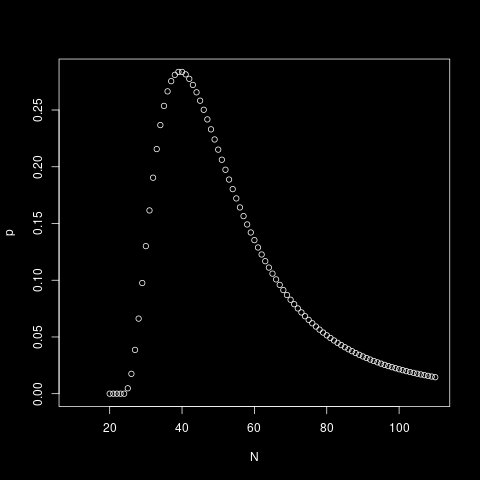
\includegraphics[scale=0.25]{Wildlife-neg.png}
 \end{minipage}
\end{enumerate}
\end{frame}
%-------------- end slide -------------------------------%}}}
%-------------- start slide -------------------------------%{{{ 5.24
\begin{frame}
	\begin{enumerate}
		\item[] The graph suggests to sudty the following quantity:
			\vfill
 \[
 r(N) := \frac{L(N)}{L(N-1)} =\frac{N-n}{N} \times \frac{N-a}{N-a-n+k}
 \]
 \vfill \pause
 \[
 r(N)<1 \quad\Longleftrightarrow \quad na<Nk \quad \text{i.e., $N>\frac{na}{k}$}
 \]\pause
 \vfill
 \[
\boxed{ N_e = \mathop{\arg\max} \left\{ L(N): N = \Floor{\frac{na}{k}}, \Ceil{\frac{na}{k}} \right\}}.
 \]
 \myEnd
	\end{enumerate}
\end{frame}
%-------------- end slide -------------------------------%}}}
%-------------- start slide -------------------------------%{{{ 5.25
\begin{frame}{Method of Moments Estimation}

 {\bf Rationale:~} The population moments should be close to the sample moments, i.e.,
 \[
\E(Y^k) \approx \frac{1}{n}\sum_{i=1}^ny_i^k , \quad k=1,2,3,\cdots.
 \]

 \vfill
{\bf\noindent Definition 5.2.3.~}  For a random sample of size $n$ from the discrete (resp. continuous) population/pdf $p_X(k;\theta_1,\cdots,\theta_s)$ (resp. $f_Y(y;\theta_1,\cdots,\theta_s)$), solutions to
\[
\begin{cases}
 \E(Y)  = \frac{1}{n}\sum_{i=1}^n y_i \\
 \qquad \vdots\\
 \E(Y^s)  = \frac{1}{n}\sum_{i=1}^n y_i^s \\
\end{cases}
\]
which are denoted by $\theta_{1e},\cdots, \theta_{se}$,
are called the {\bf method of moments estimates} of $\theta_1,\cdots, \theta_s$.
\end{frame}
%-------------- end slide -------------------------------%}}}
%-------------- start slide -------------------------------%{{{ 5.26
\begin{frame}{Examples for MME}
 MME is often the same as MLE:\\
 \vfill
 \begin{enumerate}
  \item[E.g. 1.] Normal distribution: $f_Y(y;\mu,\sigma^2)= \frac{1}{\sqrt{2\pi} \sigma} e^{-\frac{(y-\mu)^2}{2\sigma^2}}$, $y\in\R$.
  \vfill
  \[
  \begin{cases}
   \displaystyle
   \mu  = \E(Y) = \frac{1}{n} \sum_{i=1}^n y_i = \bar{y}\\
   \displaystyle
   \sigma^2 + \mu^2  = \E(Y^2) = \frac{1}{n} \sum_{i=1}^n y_i^2 \\
  \end{cases}
  \quad\Rightarrow\quad
  \begin{cases}
   \displaystyle
   \mu_e  =  \bar{y}\\
   \displaystyle
   \sigma_e^2 = \frac{1}{n} \sum_{i=1}^n y_i^2 -\mu_e^2 \\
   \phantom{\sigma_e^2 }= \frac{1}{n}\sum_{i=1}^n\left(y_i-\bar{y}\right)^2
  \end{cases}
  \]
\vfill
More examples when MLE coincides with MME: Poisson, Exponential, Geometric.
\end{enumerate}
\end{frame}
%-------------- end slide -------------------------------%}}}
%-------------- start slide -------------------------------%{{{ 5.27
\begin{frame}
MME is often much more tractable than MLE:\\
 \vfill
 \begin{enumerate}
  \item[E.g. 2.] Gamma distribution\footnote{Check Theorem 4.6.3 on p. 269 for mean and variance}: $f_Y(y;r, \lambda)= \frac{\lambda^r}{\Gamma(r)} y^{r-1} e^{-\lambda y}$ for $y\ge 0$.
  \[
  \begin{cases}
   \displaystyle
   \frac{r}{\lambda} = \E(Y) = \frac{1}{n} \sum_{i=1}^n y_i = \bar{y}\\
   \displaystyle
   \frac{r}{\lambda^2} + \frac{r^2}{\lambda^2}  = \E(Y^2) = \frac{1}{n} \sum_{i=1}^n y_i^2 \\
  \end{cases}
  \quad\Rightarrow\quad
  \begin{cases}
   \displaystyle
   r_e = \frac{\bar{y}^2}{\hat{\sigma}^2} \\[1em]
   \displaystyle
   \lambda_e = \frac{\bar{y}}{\hat{\sigma}^2} = \frac{r_e}{\bar{y}}
  \end{cases}
  \]
  where $\bar{y}$ is the sample mean and $\hat{\sigma}^2$ is the sample variance: $\hat{\sigma}^2:= \frac{1}{n}\sum_{i=1}^n(y_i-\bar{y})^2$.
  \vfill
 Comments: MME for $\lambda$ is consistent with MLE when $r$ is known.
 \end{enumerate}
 \end{frame}
%-------------- end slide -------------------------------%}}}
%-------------- start slide -------------------------------%{{{ 5.28
\begin{frame}
  Another tractable example for MME, while less tractable for MLE: \\
  \vfill
  \begin{enumerate}
  \item[E.g. 3.] Neg. binomial distribution: $p_X(k;p,r)={k+r-1\choose k}(1-p)^k p^r$, $k=0,1,\cdots$.
 \[
  \begin{cases}
   \displaystyle
   \frac{r(1-p)}{p} =\E(X) = \bar{k}\\
   \displaystyle
   \frac{r(1-p)}{p^2}= \text{Var}(X) =  \hat{\sigma}^2
  \end{cases}
  \quad\Rightarrow\quad
  \begin{cases}
   \displaystyle
   p_e = \frac{\bar{k}}{\hat{\sigma}^2} \\[1em]
   \displaystyle
   r_e = \frac{\bar{k}^2}{\hat{\sigma}^2-\bar{k}}
  \end{cases}
  \]
 \end{enumerate}

\end{frame}
%-------------- end slide -------------------------------%}}}
%-------------- start slide -------------------------------%{{{ 5.29
\begin{frame}
\begin{center}
 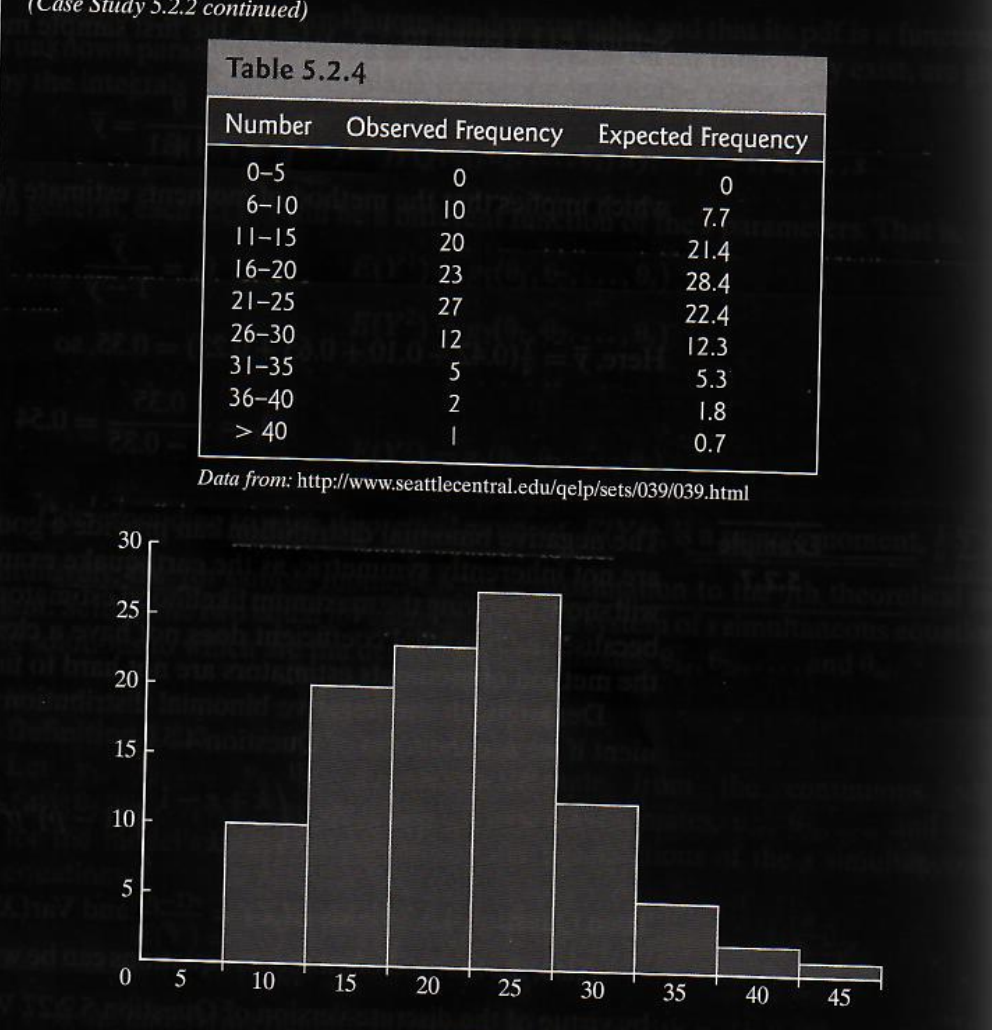
\includegraphics[scale=0.22]{figure-5-2-2-neg.png}\\
 {$r_e=12.74$ and $p_e=0.391$.}
\end{center}
\end{frame}
%-------------- end slide -------------------------------%}}}
%-------------- start slide -------------------------------%{{{ 5.30
\begin{frame}
  \begin{enumerate}
  \item[E.g. 4.] $f_Y(y;\theta) = \frac{2y}{\theta^2}$ for $y\in [0,\theta]$.\\[2em]
  \[
  \overline{y} = \E[Y] = \int_0^\theta \frac{2y^2}{\theta^2}\ud y = \frac{2}{3} \frac{y^3}{\theta^2}\bigg|_{y=0}^{y=\theta} = \frac{2}{3}\theta.
  \]
  \[
  \Downarrow
  \]
  \[
  \boxed{\theta_e = \frac{3}{2}\overline{y}.}
  \]
 \end{enumerate}

\end{frame}
%-------------- end slide -------------------------------%}}}
